\chapter{Validación Experimental y Resultados de Precertificación}
\label{ch:precompliance_results}

Una vez descrito el diseño hardware del DCU (Capítulo \ref{ch:hardware_design}) y de su fuente de alimentación HV/HF (Capítulo \ref{HV_HF_PSU}), el siguiente paso consiste en verificar que el prototipo es capaz de superar la batería de ensayos tipo (\textit{Type Tests}) exigida para su homologación. Antes de acudir a la homologación definitiva en un laboratorio acreditado, se ha llevado a cabo una campaña de \textbf{precertificación} (\textit{pre-compliance}) en un centro de ensayos externo, con el objetivo de detectar de forma temprana posibles incumplimientos (especialmente en materia de EMC) y poder corregirlos en una fase del diseño en la que todavía resulta viable modificar el hardware sin un impacto elevado en coste y plazos.
% NOTA: confirmar si se puede nombrar explícitamente al centro de ensayos (ITA, Instituto Tecnológico de Aragón) y la fecha de la campaña.

Los ensayos se agrupan en ocho familias: aislamiento, perturbaciones radioeléctricas (emisiones), inmunidad electromagnética, ensayos eléctricos, ensayos mecánicos, ensayos climáticos, seguridad eléctrica y señalización PLC. La Tabla \ref{tab:familias_ensayos} resume la naturaleza del resultado que proporciona cada una de ellas. Este capítulo se centra en aquellos ensayos que proporcionan un \textbf{resultado cuantitativo} (fundamentalmente capturas del analizador de espectro y valores medidos frente a un límite normativo), mientras que los ensayos cuyo resultado se reduce a la verificación de un criterio de funcionamiento (``pasa/no pasa'') se describen de forma más breve, indicando en qué consisten y qué situación real pretenden simular.

\begin{table}[!h]
\centering
\small
\begin{tabular}{|p{3.4cm}|p{5.6cm}|p{5.2cm}|}
\hline
\textbf{Familia de ensayos} & \textbf{Normas principales} & \textbf{Tipo de resultado} \\ \hline
Perturbaciones radioeléctricas & EN 55032, EN 61000-3-2, EN 61000-3-3 & Cuantitativo (espectros y valores medidos frente a límite) \\ \hline
Señalización PLC & EN 50065-1 & Cuantitativo (espectro de la señal PLC y emisiones fuera de banda) \\ \hline
Aislamiento & EN 60255-27, EN 62368-1 & Cuantitativo (resistencia de aislamiento) y verificación de ausencia de descarga disruptiva \\ \hline
Eléctricos & EN 61000-4-11, EN 62052-11, EN 62053-23 & Criterio de funcionamiento (A/B) \\ \hline
Inmunidad electromagnética & Serie EN 61000-4-x & Criterio de funcionamiento (A/B) \\ \hline
Mecánicos & EN 60529, ETSI EN 300 019-2-2 & Pasa / no pasa \\ \hline
Climáticos & Serie EN 60068-2-x & Criterio de funcionamiento (A/B) \\ \hline
Seguridad eléctrica & EN 62368-1 & Pasa / no pasa \\ \hline
\end{tabular}
\caption{Familias de ensayos tipo aplicables al DCU y naturaleza del resultado obtenido en cada una de ellas.}
\label{tab:familias_ensayos}
\end{table}

\section{Estudio de Sensibilidad de la Comunicación PLC}
\label{sec:sensibilidad_plc}

Los ensayos normativos que se presentan en el resto de este capítulo verifican que el equipo no supera los límites de emisión establecidos y que tolera las perturbaciones externas, pero no cuantifican directamente la calidad de la comunicación PLC ni el efecto que tiene sobre ella el ruido generado por el propio equipo. Por este motivo, y como complemento a la campaña de precertificación, se ha diseñado un \textbf{estudio de sensibilidad de la comunicación PLC}, realizado en los laboratorios propios de la empresa. Su objetivo es determinar cuánta atenuación admite el canal PLC antes de que la comunicación comience a degradarse, comparando el comportamiento del DCU con el de equipos de referencia.

Este estudio constituye la validación experimental más directa de la hipótesis central del trabajo: colocar la frecuencia de conmutación de la fuente de alimentación por encima de las bandas PLC (Secciones \ref{subsec:topologias_alta_frecuencia_tension} y \ref{subsec:requisitos_emc_psu}) mejora de forma cuantificable la calidad de la comunicación frente a equipos cuya fuente conmuta dentro de dichas bandas.

Además de la sensibilidad del enlace, el estudio persigue caracterizar la \textbf{coexistencia entre la fuente conmutada y la comunicación PLC} dentro del propio equipo: es decir, cuantificar en qué medida el ruido que genera la fuente de alimentación (y el resto de la electrónica) en la banda PLC se acopla al receptor del propio módem y reduce el margen de enlace disponible. Dado que el DCU y su módem comparten los mismos terminales de red, este ruido llega al receptor sin ninguna atenuación, a diferencia de la señal procedente del extremo remoto, por lo que su efecto se hace más evidente cuanto mayor es la atenuación del canal.

\subsection{Montaje Experimental}
\label{subsec:montaje_sensibilidad}

El montaje, representado en la Figura \ref{fig:montaje_sensibilidad_plc}, se basa en dos redes de estabilización de impedancia de línea (\textit{Line Impedance Stabilization Network, LISN}). Cada lado del montaje se alimenta de la red a través de su propia LISN, que presenta al equipo una impedancia de red definida y repetible y filtra el ruido procedente de la red del laboratorio. De esta forma, a las frecuencias de la señal PLC, ambos lados quedan aislados entre sí y respecto a la instalación del laboratorio. Las salidas de RF de las dos LISN se interconectan a través de un \textbf{atenuador variable} de 50 $\Omega$, que pasa a ser el único camino de acoplamiento de la señal PLC entre ambos lados. Esto permite emular de forma controlada la atenuación que sufriría la señal en una red de baja tensión real.

\begin{itemize}
    \item \textbf{Lado A:} se conecta un equipo de comunicación PLC ya validado, una placa de evaluación \textbf{PL460-EK} de Microchip, que actúa como extremo remoto del enlace.
    \item \textbf{Lado B:} se conectan el equipo bajo ensayo (\textit{Equipment Under Test, EUT}) y una segunda placa PL460-EK que actúa como receptor de referencia. Al compartir la misma LISN, ambos equipos están sometidos exactamente a las mismas condiciones de canal (atenuación, impedancia y ruido), lo que permite comparar directamente sus prestaciones.
\end{itemize}

Dado que el DCU integra el mismo módem PL460 que la placa de evaluación (Sección \ref{subsec:afe_driver}), las diferencias que se observen entre ambos no pueden atribuirse al propio módem, sino a la implementación del equipo: el ruido generado por su fuente de alimentación y su electrónica digital, el circuito de acoplamiento a la red y el diseño de la PCB.
% NOTA: comprobar que las LISN empleadas son válidas por debajo de 150 kHz (p. ej. redes en V de 50 uH + 5 ohm, definidas a partir de 9 kHz en CISPR 16-1-2); una LISN de 50 uH / 50 ohm pensada solo para 150 kHz - 30 MHz presenta una impedancia menor en la banda CENELEC-A y el condensador de acoplamiento de su salida de RF puede introducir atenuación adicional. Medir también la pérdida de inserción del camino LISN-LISN con el atenuador a 0 dB, para sumarla a la atenuación nominal del atenuador.
% NOTA: indicar fase de inyección, canal PRIME (canal 1, CENELEC-A) y versión de firmware / herramienta de test usada en las PL460-EK.

\begin{figure}[htbp]
    \centering
    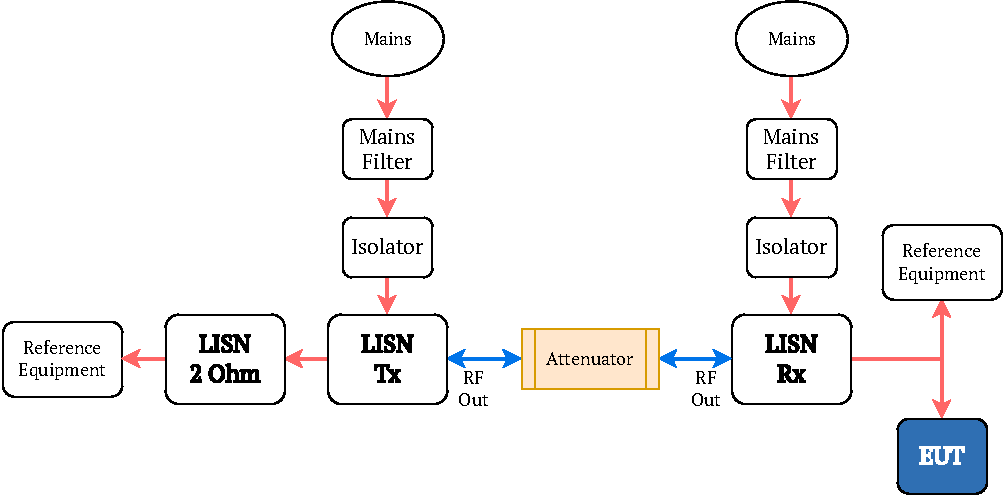
\includegraphics[width=0.9\textwidth]{Imagenes/montaje_sensibilidad_plc.pdf}
    \caption{Esquema del montaje del estudio de sensibilidad PLC: dos LISN con sus salidas de RF interconectadas a través de un atenuador variable, con la PL460-EK remota en el lado A y el EUT junto a la PL460-EK de referencia en el lado B.}
    \label{fig:montaje_sensibilidad_plc}
\end{figure}

\begin{figure}[htbp]
    \centering
    % \includegraphics[width=0.8\textwidth]{Imagenes/foto_montaje_sensibilidad_plc.jpg}
    \caption{Montaje del estudio de sensibilidad PLC en el laboratorio.}
    \label{fig:foto_montaje_sensibilidad_plc}
\end{figure}

\subsection{Configuraciones Evaluadas}
\label{subsec:configuraciones_sensibilidad}

Para aislar la contribución de cada elemento, el estudio se repite en las configuraciones recogidas en la Tabla \ref{tab:configuraciones_sensibilidad}. En todas ellas el extremo remoto del lado A es la misma PL460-EK.

\begin{table}[!h]
\centering
\small
\begin{tabular}{|p{3.2cm}|p{5.4cm}|p{5.6cm}|}
\hline
\textbf{Configuración} & \textbf{Equipos en el lado B} & \textbf{Finalidad} \\ \hline
C1: Referencia & PL460-EK de referencia, con el EUT desconectado & Sensibilidad del módem sin la influencia de otros equipos (línea base). \\ \hline
C2: Referencia junto al EUT & PL460-EK de referencia, con el EUT alimentado pero sin transmitir & Efecto del ruido del EUT sobre un equipo vecino conectado a la misma red. \\ \hline
C3: EUT & DCU desarrollado en este trabajo (fuente conmutando por encima de 500 kHz) & Calidad de transmisión y recepción del propio DCU frente a la referencia. \\ \hline
C4: Equipo con fuente comercial & Equipo PLC alimentado con una fuente comercial que conmuta dentro de la banda PLC & Mejora aportada por una fuente que conmuta fuera de las bandas PLC. \\ \hline
\end{tabular}
\caption{Configuraciones evaluadas en el estudio de sensibilidad PLC.}
\label{tab:configuraciones_sensibilidad}
\end{table}
% NOTA: C2 es opcional; eliminarla si finalmente no se realiza. Describir el equipo de C4 (sin nombrar al fabricante si no procede) y su frecuencia de conmutación.

\subsection{Procedimiento y Métricas Evaluadas}
\label{subsec:procedimiento_sensibilidad}

Partiendo de una atenuación nula, la atenuación del canal se incrementa en escalones (más finos en las proximidades del umbral de pérdida de tramas). En cada escalón se transmite un número fijo de tramas, de longitud y esquema de modulación constantes, y se registran las métricas que proporciona el propio módem receptor. La medida se realiza en ambos sentidos del enlace, ya que evalúan aspectos distintos del equipo:

\begin{itemize}
    \item \textbf{Transmisión (lado B $\rightarrow$ lado A):} evalúa la calidad de la señal inyectada por el equipo en la red, que depende de su nivel de salida, de su circuito de acoplamiento y de la impedancia que presenta el propio equipo en la banda PLC.
    \item \textbf{Recepción (lado A $\rightarrow$ lado B):} evalúa la sensibilidad del receptor, que es la más afectada por el ruido que el propio equipo genera en la banda PLC y que se suma a la señal atenuada que llega desde el extremo remoto.
\end{itemize}

El procedimiento se repite para los distintos esquemas de modulación de PRIME (DBPSK, DQPSK y D8PSK, con y sin FEC), ya que cada uno requiere una SNR mínima distinta para decodificarse correctamente.
% NOTA: confirmar las modulaciones realmente ensayadas (y los modos robustos si se usa PRIME 1.4), el número de tramas por escalón, su longitud y el tamaño del escalón de atenuación.

En cada escalón se registran las siguientes métricas:

\begin{itemize}
    \item \textbf{Indicador de intensidad de señal recibida (\textit{Received Signal Strength Indicator, RSSI}):} nivel de señal medido en el receptor. En condiciones ideales disminuye linealmente con la atenuación introducida; cuando la señal se aproxima al ruido de fondo, el RSSI deja de disminuir y se estabiliza en el nivel de ruido presente en la banda, lo que permite estimar el ruido que aporta cada configuración.
    \item \textbf{SNR:} relación señal a ruido estimada por el propio módem sobre las tramas recibidas. Es la métrica que determina directamente qué esquemas de modulación puede utilizar el enlace.
    \item \textbf{Tasa de error de trama (\textit{Frame Error Rate, FER}):} porcentaje de tramas enviadas que no se reciben correctamente, $\text{FER} = \left(1 - N_{rx}/N_{tx}\right) \cdot 100\%$.
\end{itemize}

A partir de estas medidas se definen dos puntos característicos para cada configuración: la \textbf{atenuación máxima sin pérdida de tramas} ($A_{0}$, última atenuación con $\text{FER} = 0\%$) y la \textbf{atenuación de pérdida total del enlace} ($A_{100}$, primera atenuación con $\text{FER} = 100\%$). La diferencia de $A_{0}$ entre dos configuraciones expresa, en decibelios, el margen adicional de enlace que aporta una sobre la otra, directamente trasladable a la atenuación adicional (longitud de línea, número de derivaciones o cargas conectadas) que el enlace puede tolerar en una red real.
% NOTA: si se prefiere, definir el umbral con un FER distinto de 0 % (p. ej. 1 % o 10 %).

\subsection{Resultados}
\label{subsec:resultados_sensibilidad}

Las Figuras \ref{fig:fer_vs_atenuacion}, \ref{fig:rssi_vs_atenuacion} y \ref{fig:snr_vs_atenuacion} muestran la evolución de las métricas con la atenuación del canal para cada configuración, y la Tabla \ref{tab:resultados_sensibilidad} resume los puntos característicos obtenidos.

\begin{figure}[htbp]
    \centering
    % \includegraphics[width=0.8\textwidth]{Imagenes/fer_vs_atenuacion.pdf}
    \caption{Tasa de error de trama (FER) en función de la atenuación del canal para cada configuración.}
    \label{fig:fer_vs_atenuacion}
\end{figure}

\begin{figure}[htbp]
    \centering
    % \includegraphics[width=0.8\textwidth]{Imagenes/rssi_vs_atenuacion.pdf}
    \caption{RSSI en función de la atenuación del canal para cada configuración.}
    \label{fig:rssi_vs_atenuacion}
\end{figure}

\begin{figure}[htbp]
    \centering
    % \includegraphics[width=0.8\textwidth]{Imagenes/snr_vs_atenuacion.pdf}
    \caption{SNR en función de la atenuación del canal para cada configuración.}
    \label{fig:snr_vs_atenuacion}
\end{figure}

\begin{table}[!h]
\centering
\small
\begin{tabular}{|p{3.4cm}|p{1.9cm}|p{1.6cm}|p{1.6cm}|p{2.2cm}|p{2.0cm}|}
\hline
\textbf{Configuración} & \textbf{Sentido} & \textbf{$A_{0}$ (dB)} & \textbf{$A_{100}$ (dB)} & \textbf{RSSI en $A_{0}$ (dB$\mu$V)} & \textbf{SNR en $A_{0}$ (dB)} \\ \hline
\multirow{2}{3.4cm}{C1: Referencia} & TX & -- & -- & -- & -- \\ \cline{2-6}
 & RX & -- & -- & -- & -- \\ \hline
\multirow{2}{3.4cm}{C2: Referencia junto al EUT} & TX & -- & -- & -- & -- \\ \cline{2-6}
 & RX & -- & -- & -- & -- \\ \hline
\multirow{2}{3.4cm}{C3: EUT} & TX & -- & -- & -- & -- \\ \cline{2-6}
 & RX & -- & -- & -- & -- \\ \hline
\multirow{2}{3.4cm}{C4: Fuente comercial} & TX & -- & -- & -- & -- \\ \cline{2-6}
 & RX & -- & -- & -- & -- \\ \hline
\end{tabular}
\caption{Puntos característicos del estudio de sensibilidad PLC para cada configuración y sentido del enlace.}
\label{tab:resultados_sensibilidad}
\end{table}

Para relacionar estas diferencias de sensibilidad con su origen, se mide además con el analizador de espectro el ruido de fondo presente en la banda CENELEC-A en la salida de RF de la LISN del lado B, con la transmisión PLC desactivada, de forma que la medida recoge exclusivamente la contribución de la fuente de alimentación y del resto de la electrónica del equipo. La Figura \ref{fig:ruido_banda_eut_vs_comercial} compara este ruido para el EUT (C3) y para el equipo con fuente comercial (C4). La diferencia entre el nivel de la señal PLC transmitida (Figura \ref{fig:espectro_tx_plc}) y este ruido de fondo representa la relación señal a ruido disponible en bornes del propio equipo, y permite verificar experimentalmente que situar la frecuencia de conmutación de la fuente por encima de 500 kHz evita que esta degrade la recepción PLC, mientras que una fuente que conmuta dentro de la banda eleva el ruido de fondo y reduce directamente el margen de enlace.

\begin{figure}[htbp]
    \centering
    % \includegraphics[width=0.8\textwidth]{Imagenes/ruido_banda_eut_vs_comercial.png}
    \caption{Ruido de fondo en la banda CENELEC-A con la transmisión PLC desactivada: EUT (fuente conmutando por encima de 500 kHz) frente al equipo con fuente comercial conmutando dentro de la banda.}
    \label{fig:ruido_banda_eut_vs_comercial}
\end{figure}

% Pendiente: análisis de resultados, relacionando el ruido de fondo de cada configuración con el RSSI de saturación y con A_0 (diferencia de A_0 entre C3 y C1 -> penalización del diseño frente a la referencia; entre C3 y C4 -> mejora aportada por la fuente fuera de banda; entre C2 y C1 -> ruido que el EUT inyecta a equipos vecinos).

\section{Metodología y Configuración de los Ensayos de Precertificación}
\label{sec:metodologia_ensayos}

\subsection{Equipo Bajo Ensayo y Montaje General}
\label{subsec:eut_montaje}

El EUT es el prototipo del DCU descrito en los capítulos anteriores, con unas dimensiones aproximadas de $200 \times 120 \times 75$ mm y un peso estimado de medio kilogramo. Un requisito fundamental de la especificación del cliente es que \textbf{todos los ensayos de una misma familia se realicen sobre el mismo prototipo}, identificando debidamente tanto la versión de hardware como la de software, de forma que los resultados no puedan atribuirse a diferencias entre unidades.

Durante los ensayos, el EUT se alimenta desde la red trifásica ($L1/L2/L3/N$, denominadas $R/S/T/N$ en los informes del laboratorio) y todos sus puertos se mantienen conectados y estimulados de forma representativa de su operación real en un CT:

\begin{itemize}
    \item \textbf{Terminales de alimentación ($L1/L2/L3/N$):} a la misma red se conecta un nodo de servicio auxiliar sobre la fase $L1$, con el que el DCU (actuando como Nodo Base PRIME) mantiene una comunicación PLC constante.
    \item \textbf{Terminales de medida de corriente:} se excitan con una corriente alterna constante de entre 3 y 5 A por fase, con un ángulo de fase fijo respecto a la tensión correspondiente, de forma que el bloque de metrología (Sección \ref{sec:metrologia_trifasica}) esté midiendo de forma continua durante el ensayo.
    \item \textbf{Puertos Ethernet (WAN y LAN):} se conectan a un ordenador auxiliar con dos interfaces de red, desde el que se mantienen sesiones de \textit{ping} continuas (una petición por segundo) hacia ambos puertos y desde el que se accede a la interfaz web de configuración del equipo.
    \item \textbf{Entradas y salidas digitales:} las entradas se mantienen estimuladas con una fuente de laboratorio (12 V durante los ensayos de emisión) y las salidas se mantienen activadas.
\end{itemize}

\begin{figure}[htbp]
    \centering
    % \includegraphics[width=0.8\textwidth]{Imagenes/setup_general_ensayos.png}
    \caption{Montaje general del EUT durante la campaña de precertificación, con el nodo de servicio auxiliar, el estímulo de los terminales de corriente y el ordenador de supervisión conectado a los puertos Ethernet.}
    \label{fig:setup_general_ensayos}
\end{figure}

\subsection{Supervisión del Funcionamiento y Criterios de Aceptación}
\label{subsec:supervision_criterios}

Para los ensayos que se evalúan mediante un criterio de funcionamiento, se aplican los criterios A y B ya definidos en la Sección \ref{subsec:requisitos_emc_psu}. La verificación de que el equipo ``continúa funcionando correctamente'' se concreta en la supervisión de cada una de sus funciones principales:

\begin{itemize}
    \item \textbf{Comunicación PLC:} se comprueba que el nodo de servicio auxiliar permanece registrado en la red PRIME. Dado que este nodo pierde la sincronización tras 4 segundos sin recibir la baliza (\textit{beacon}) del Nodo Base, cualquier interrupción de la comunicación provoca un nuevo registro, detectable porque cambia la hora del último registro respecto a la inicial.
    \item \textbf{Metrología:} se configura un periodo de medida de 5 segundos y se verifica que las medidas siguen llegando periódicamente y que su fluctuación tras el ensayo es inferior a $0,01$.
    \item \textbf{Ethernet:} las sesiones de \textit{ping} deben mantenerse durante todo el ensayo (criterio A) o reanudarse inmediatamente al finalizar la perturbación (criterio B). En ningún caso se admite un reinicio del SoM.
    \item \textbf{Entradas y salidas digitales:} tras el ensayo se comprueba que las entradas detectan correctamente los niveles alto (9 V y 50 V) y bajo, y que las salidas conmutan correctamente, verificando la continuidad entre sus contactos.
\end{itemize}

\subsection{Modo de Operación Durante los Ensayos de Emisión}
\label{subsec:modo_operacion_emisiones}

Para que la medida de emisiones sea representativa del peor caso de funcionamiento, durante los ensayos de perturbaciones radioeléctricas el módem PLC se configura en un \textbf{modo de transmisión continua}, enviando paquetes de forma ininterrumpida por los terminales de red. La transmisión se configura en el canal 1 de PRIME, situado dentro de la banda CENELEC-A (Sección \ref{subsec:marcos_espectrales}) y, por tanto, por debajo de los 150 kHz a partir de los cuales comienza el rango de medida de las emisiones conducidas. De esta forma, la señal PLC útil no enmascara el ruido generado por el propio equipo, mientras que la fuente de alimentación y la electrónica digital operan con su carga máxima. Previamente a los ensayos se verifica con el analizador de espectro que el espectro de transmisión PLC es correcto (nivel ni demasiado bajo ni demasiado alto y bajo ruido fuera de banda).

\section{Ensayos de Perturbaciones Radioeléctricas (Emisiones)}
\label{sec:ensayos_emisiones}

Estos ensayos cuantifican el ruido electromagnético que el propio equipo genera y, por tanto, constituyen la validación experimental más directa de las decisiones de diseño de la fuente HV/HF descritas en el Capítulo \ref{HV_HF_PSU}. En todos ellos se exige el cumplimiento de la \textbf{Clase B} (entorno residencial), más restrictiva que la Clase A (entorno industrial), a pesar de que el equipo se instala en un CT.

\subsection{Emisiones Conducidas en los Terminales de Alimentación AC (EN 55032)}
\label{subsec:emisiones_conducidas_ac}

\subsubsection*{Descripción del ensayo}

El ensayo mide la tensión de perturbación que el equipo inyecta en la red de alimentación en el rango de 150 kHz a 30 MHz. El EUT se conecta a la red a través de una LISN (denominada red artificial de alimentación, \textit{Artificial Mains Network}, en la terminología de EN 55032), que presenta una impedancia normalizada entre cada conductor y el plano de tierra de referencia, desacopla el ruido procedente de la red del laboratorio y permite extraer la tensión de perturbación hacia el receptor de medida. El ensayo se realiza con conexión trifásica, midiendo por separado cada uno de los cuatro conductores ($L1$, $L2$, $L3$ y $N$).

La medida se realiza en dos pasos: en primer lugar, un barrido rápido con detector de pico y retención de máximos (\textit{max-hold}) permite identificar las frecuencias críticas; a continuación, sobre dichas frecuencias se realiza la medida final con los detectores de cuasi-pico (QP) y promedio (AV), con un ancho de banda de resolución de 9 kHz, que son los que se comparan con los límites de la Tabla \ref{tab:requisitos_emc_emisiones}.

\begin{figure}[htbp]
    \centering
    % \includegraphics[width=0.8\textwidth]{Imagenes/setup_emisiones_conducidas.png}
    \caption{Montaje del ensayo de emisiones conducidas en los terminales de alimentación AC según EN 55032.}
    \label{fig:setup_emisiones_conducidas}
\end{figure}

\subsubsection*{Resultados}

La Figura \ref{fig:ec_ac} muestra los espectros de emisión conducida obtenidos en cada uno de los conductores de alimentación, junto con los límites de Clase B de cuasi-pico y promedio.

\begin{figure}[htbp]
    \centering
    \begin{subfigure}[b]{0.48\textwidth}
        \centering
        % \includegraphics[width=\linewidth]{Imagenes/ec_ac_L1.png}
        \caption{Fase $L1$ ($R$).}
        \label{fig:ec_ac_L1}
    \end{subfigure}
    \hfill
    \begin{subfigure}[b]{0.48\textwidth}
        \centering
        % \includegraphics[width=\linewidth]{Imagenes/ec_ac_L2.png}
        \caption{Fase $L2$ ($S$).}
        \label{fig:ec_ac_L2}
    \end{subfigure}

    \vspace{0.4cm}
    \begin{subfigure}[b]{0.48\textwidth}
        \centering
        % \includegraphics[width=\linewidth]{Imagenes/ec_ac_L3.png}
        \caption{Fase $L3$ ($T$).}
        \label{fig:ec_ac_L3}
    \end{subfigure}
    \hfill
    \begin{subfigure}[b]{0.48\textwidth}
        \centering
        % 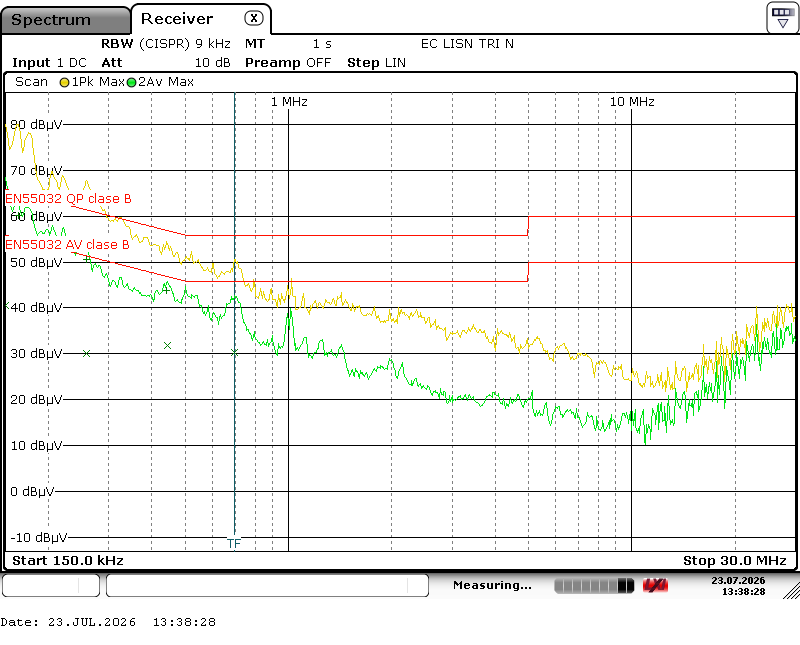
\includegraphics[width=\linewidth]{Imagenes/ec_ac_N.png}
        \caption{Neutro ($N$).}
        \label{fig:ec_ac_N}
    \end{subfigure}
    \caption{Espectros de emisión conducida (150 kHz -- 30 MHz) en los terminales de alimentación AC, frente a los límites de Clase B de EN 55032.}
    \label{fig:ec_ac}
\end{figure}

La Tabla \ref{tab:resultados_ec_ac} recoge las frecuencias críticas identificadas y el margen obtenido respecto a cada límite (un margen positivo indica que la emisión se encuentra por debajo del límite).

\begin{table}[!h]
\centering
\small
\begin{tabular}{|p{1.4cm}|p{1.6cm}|p{1.9cm}|p{1.7cm}|p{1.9cm}|p{1.7cm}|p{1.9cm}|}
\hline
\textbf{Línea} & \textbf{Frec. (MHz)} & \textbf{QP (dB$\mu$V)} & \textbf{Margen QP (dB)} & \textbf{AV (dB$\mu$V)} & \textbf{Margen AV (dB)} & \textbf{Resultado} \\ \hline
$L1$ & -- & -- & -- & -- & -- & -- \\ \hline
$L2$ & -- & -- & -- & -- & -- & -- \\ \hline
$L3$ & -- & -- & -- & -- & -- & -- \\ \hline
$N$  & -- & -- & -- & -- & -- & -- \\ \hline
\end{tabular}
\caption{Frecuencias críticas y márgenes obtenidos en el ensayo de emisiones conducidas en los terminales de alimentación AC.}
\label{tab:resultados_ec_ac}
\end{table}

% Pendiente: análisis de los resultados una vez disponibles las capturas.
El análisis de estos resultados debe centrarse especialmente en el tramo de 0,5 a 5 MHz, donde cabe esperar la contribución de la frecuencia fundamental de conmutación de la fuente (superior a 500 kHz, Sección \ref{subsec:topologia_flyback_sincrono_zvs}) y de sus primeros armónicos, así como en el tramo inicial de 150 a 500 kHz, en el que el límite es más permisivo pero en el que suele concentrarse el ruido de modo diferencial de las fuentes conmutadas.

\subsection{Emisiones Radiadas (EN 55032)}
\label{subsec:emisiones_radiadas}

\subsubsection*{Descripción del ensayo}

El ensayo de emisiones radiadas mide la intensidad de campo eléctrico generada por el equipo y sus cables en el rango de 30 MHz a 1 GHz. Se realiza en una cámara semianecoica (\textit{Semi-Anechoic Chamber, SAC}) o en un emplazamiento de ensayo en campo abierto, con el EUT situado sobre una mesa giratoria y la antena de recepción a una distancia normalizada de 10 m (o de 3 m, en cuyo caso los límites se incrementan en 10 dB, como se indicó en la Tabla \ref{tab:requisitos_emc_emisiones}). Para localizar la dirección y polarización de máxima emisión, la medida se repite con la antena en polarización horizontal y vertical y con el equipo orientado en cuatro posiciones (0°, 90°, 180° y 270°), variando además la altura de la antena. La medida final se realiza con detector de cuasi-pico y un ancho de banda de resolución de 120 kHz.

Cabe señalar que EN 55032 establece la frecuencia máxima de medida en función de la frecuencia interna más elevada del equipo: el rango de 30 MHz a 1 GHz únicamente es suficiente si dicha frecuencia no supera los 108 MHz, ampliándose hasta 2 GHz, 5 GHz o hasta un máximo de 6 GHz para frecuencias internas superiores.
% NOTA: el SoM (NXP i.MX 93, núcleo Cortex-A55) trabaja con relojes del orden de GHz, por lo que según la Tabla 1 de EN 55032 correspondería medir por encima de 1 GHz (hasta 5xFx, máx. 6 GHz). El resumen de ensayos del cliente solo recoge el rango 30 MHz - 1 GHz: confirmar con el laboratorio si se ha medido por encima de 1 GHz y, en su caso, añadir las capturas correspondientes.

\begin{figure}[htbp]
    \centering
    % \includegraphics[width=0.8\textwidth]{Imagenes/setup_emisiones_radiadas.png}
    \caption{Montaje del ensayo de emisiones radiadas en cámara semianecoica según EN 55032.}
    \label{fig:setup_emisiones_radiadas}
\end{figure}

\subsubsection*{Resultados}

Las Figuras \ref{fig:er_horizontal} y \ref{fig:er_vertical} muestran los espectros de emisión radiada obtenidos para cada polarización de antena y orientación del equipo.

\begin{figure}[htbp]
    \centering
    \begin{subfigure}[b]{0.48\textwidth}
        \centering
        % 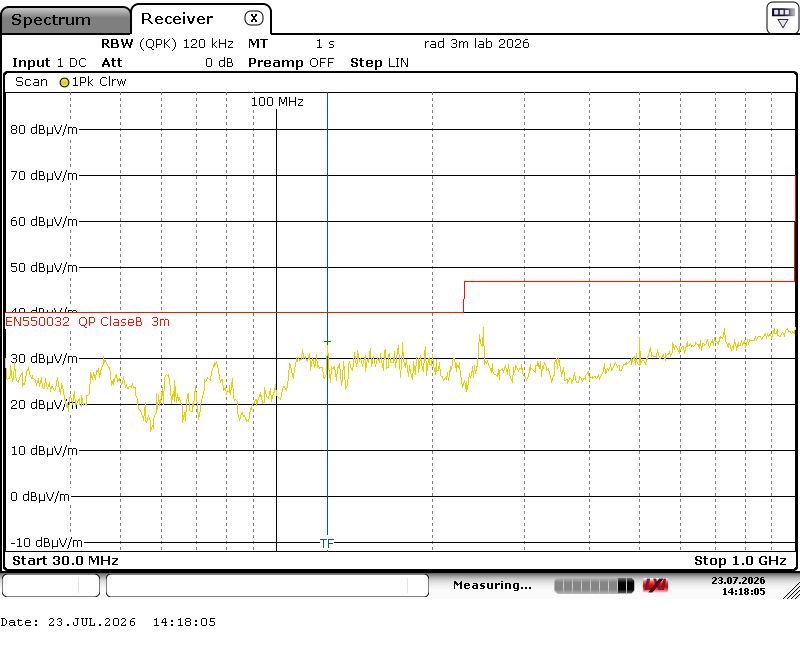
\includegraphics[width=\linewidth]{Imagenes/er_H_0.png}
        \caption{Orientación 0°.}
        \label{fig:er_H_0}
    \end{subfigure}
    \hfill
    \begin{subfigure}[b]{0.48\textwidth}
        \centering
        % 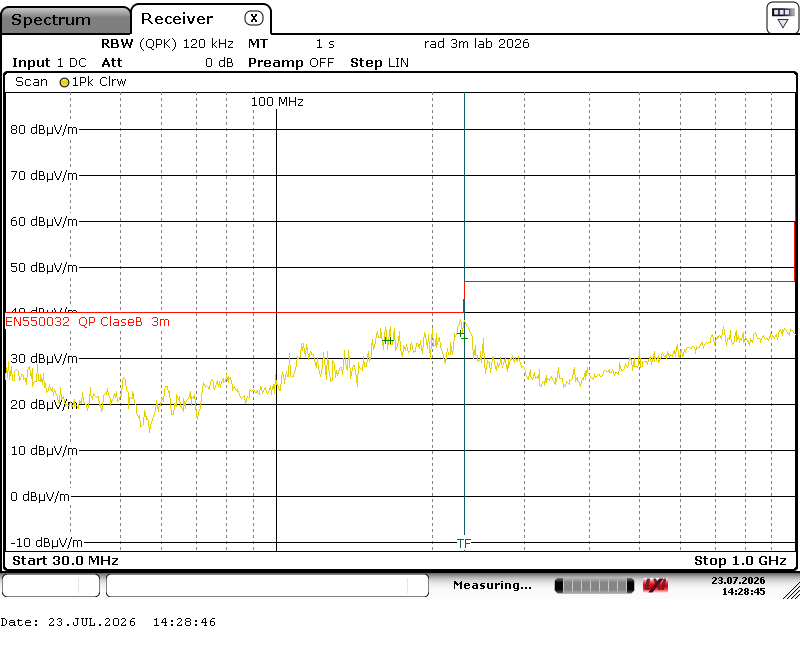
\includegraphics[width=\linewidth]{Imagenes/er_H_90.png}
        \caption{Orientación 90°.}
        \label{fig:er_H_90}
    \end{subfigure}

    \vspace{0.4cm}
    \begin{subfigure}[b]{0.48\textwidth}
        \centering
        % 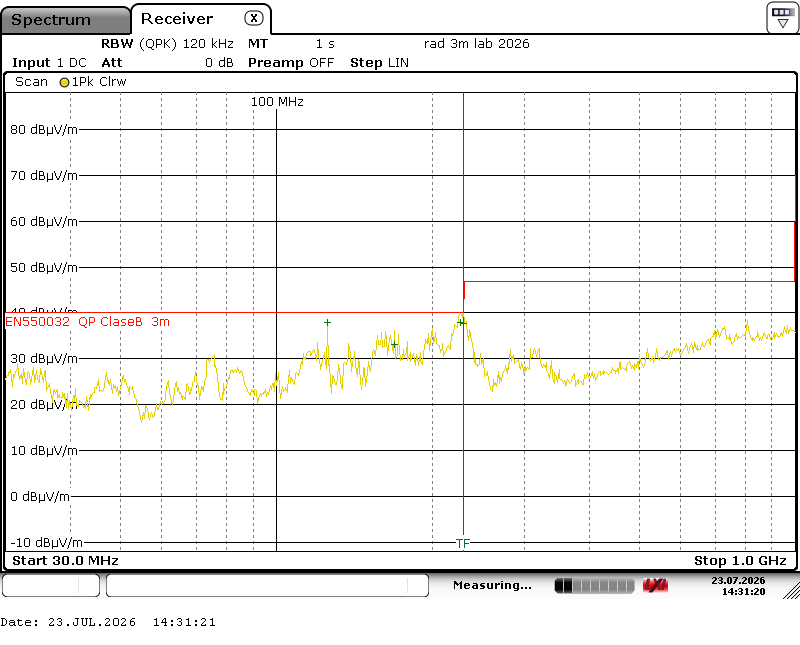
\includegraphics[width=\linewidth]{Imagenes/er_H_180.png}
        \caption{Orientación 180°.}
        \label{fig:er_H_180}
    \end{subfigure}
    \hfill
    \begin{subfigure}[b]{0.48\textwidth}
        \centering
        % 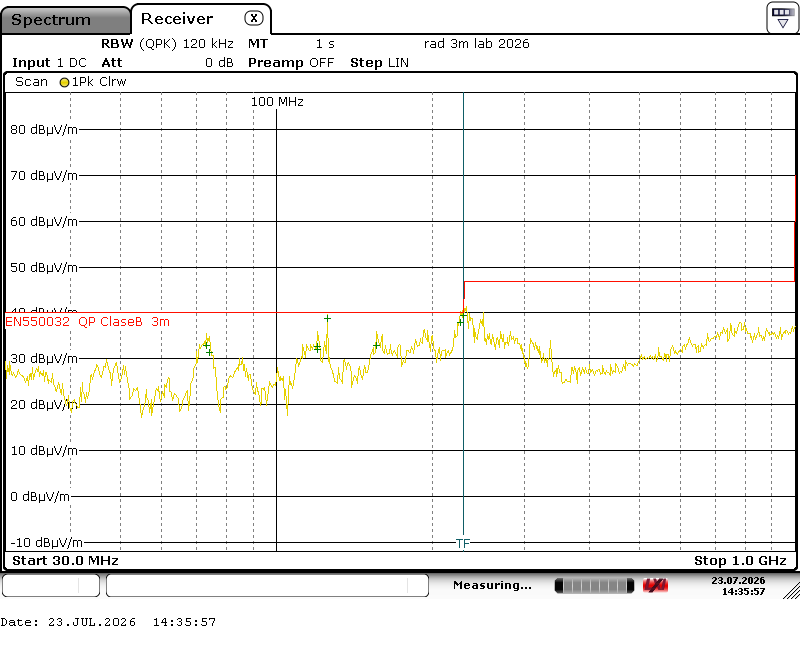
\includegraphics[width=\linewidth]{Imagenes/er_H_270.png}
        \caption{Orientación 270°.}
        \label{fig:er_H_270}
    \end{subfigure}
    \caption{Espectros de emisión radiada (30 MHz -- 1 GHz) con la antena en polarización horizontal, frente a los límites de Clase B de EN 55032.}
    \label{fig:er_horizontal}
\end{figure}

\begin{figure}[htbp]
    \centering
    \begin{subfigure}[b]{0.48\textwidth}
        \centering
        % 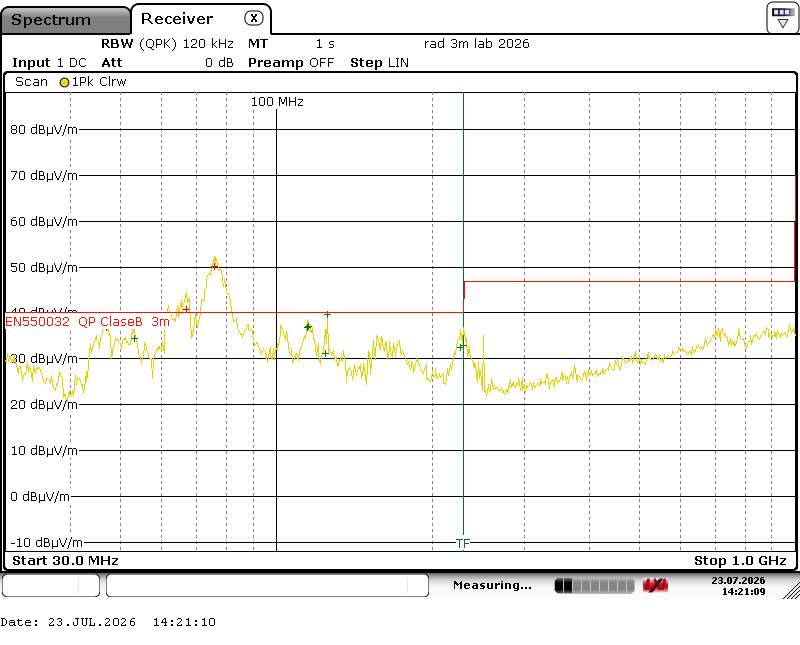
\includegraphics[width=\linewidth]{Imagenes/er_V_0.png}
        \caption{Orientación 0°.}
        \label{fig:er_V_0}
    \end{subfigure}
    \hfill
    \begin{subfigure}[b]{0.48\textwidth}
        \centering
        % 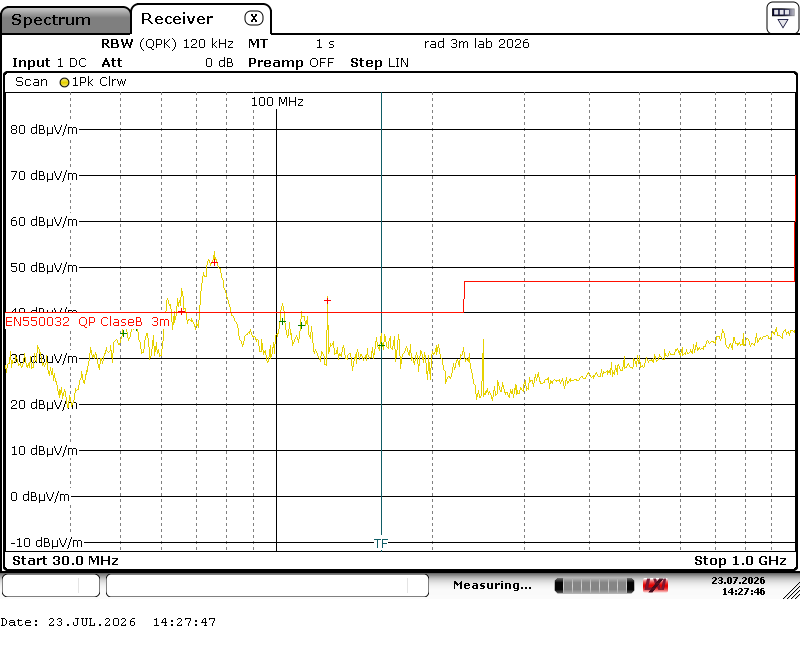
\includegraphics[width=\linewidth]{Imagenes/er_V_90.png}
        \caption{Orientación 90°.}
        \label{fig:er_V_90}
    \end{subfigure}

    \vspace{0.4cm}
    \begin{subfigure}[b]{0.48\textwidth}
        \centering
        % 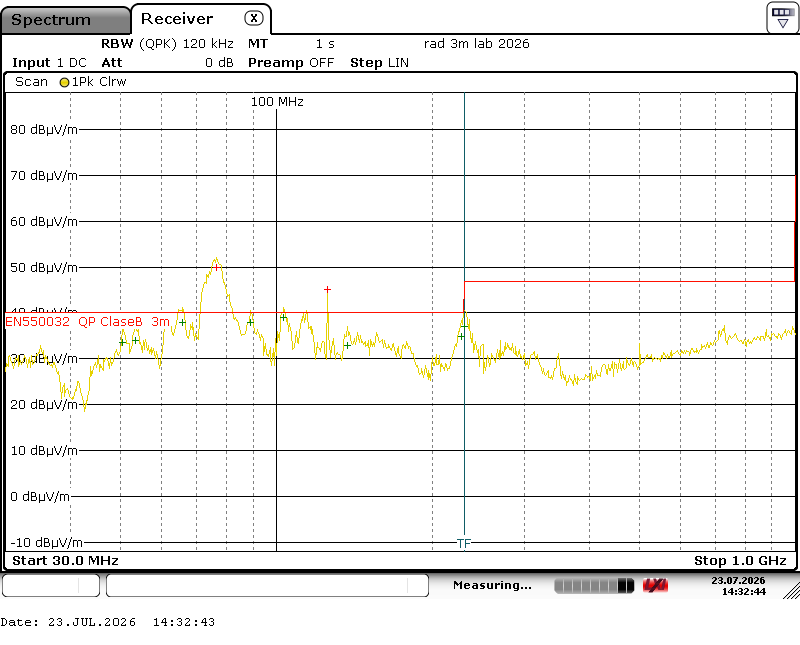
\includegraphics[width=\linewidth]{Imagenes/er_V_180.png}
        \caption{Orientación 180°.}
        \label{fig:er_V_180}
    \end{subfigure}
    \hfill
    \begin{subfigure}[b]{0.48\textwidth}
        \centering
        % 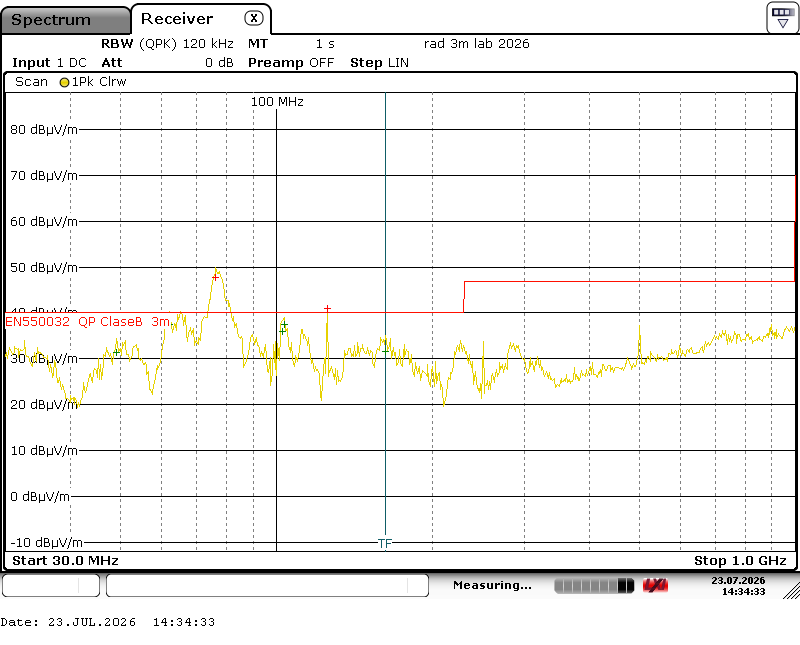
\includegraphics[width=\linewidth]{Imagenes/er_V_270.png}
        \caption{Orientación 270°.}
        \label{fig:er_V_270}
    \end{subfigure}
    \caption{Espectros de emisión radiada (30 MHz -- 1 GHz) con la antena en polarización vertical, frente a los límites de Clase B de EN 55032.}
    \label{fig:er_vertical}
\end{figure}

\begin{table}[!h]
\centering
\small
\begin{tabular}{|p{1.8cm}|p{2.5cm}|p{2.4cm}|p{2.4cm}|p{1.7cm}|p{2.0cm}|}
\hline
\textbf{Frec. (MHz)} & \textbf{Polarización} & \textbf{Orientación} & \textbf{QP medido (dB$\mu$V/m)} & \textbf{Margen (dB)} & \textbf{Resultado} \\ \hline
-- & -- & -- & -- & -- & -- \\ \hline
-- & -- & -- & -- & -- & -- \\ \hline
-- & -- & -- & -- & -- & -- \\ \hline
\end{tabular}
\caption{Frecuencias críticas y márgenes obtenidos en el ensayo de emisiones radiadas.}
\label{tab:resultados_er}
\end{table}

% Pendiente: análisis de resultados (origen probable de las emisiones críticas: relojes del SoM, DDR, PHY Ethernet, armónicos de la PSU radiados a través del cableado de red, etc.).


\subsection{Emisiones Conducidas en los Puertos de Comunicaciones (EN 55032)}
\label{subsec:emisiones_conducidas_eth}

\subsubsection*{Descripción del ensayo}

La especificación del cliente exige además medir las emisiones conducidas en los puertos Ethernet (WAN y LAN), también con límites de Clase B. En este caso se mide la perturbación en modo común (asimétrica) que el equipo inyecta en el cable de red, que actuaría como antena en la instalación real. Para ello se utiliza una red de estabilización de impedancia (\textit{Asymmetric Artificial Network, AAN}) o, alternativamente, una sonda de corriente, en el mismo rango de 150 kHz a 30 MHz. Los límites de Clase B de EN 55032 para puertos de red cableada son, medidos en tensión, de $84$--$74\ \text{dB}\mu\text{V}$ en cuasi-pico y $74$--$64\ \text{dB}\mu\text{V}$ en promedio entre 0,15 y 0,5 MHz, y de $74\ \text{dB}\mu\text{V}$ en cuasi-pico y $64\ \text{dB}\mu\text{V}$ en promedio entre 0,5 y 30 MHz.
% NOTA: estos límites proceden de la Tabla A.12 de UNE-EN 55032:2016 (puertos de red cableada, Clase B). Si el laboratorio mide con sonda de corriente, los límites equivalentes son 40--30 dBuA (QP) y 30--20 dBuA (AV) entre 0,15 y 0,5 MHz, y 30 dBuA (QP) / 20 dBuA (AV) entre 0,5 y 30 MHz. Ajustar según el método realmente empleado.

\subsubsection*{Resultados}

\begin{figure}[htbp]
    \centering
    \begin{subfigure}[b]{0.48\textwidth}
        \centering
        % \includegraphics[width=\linewidth]{Imagenes/ec_eth_WAN.png}
        \caption{Puerto WAN.}
        \label{fig:ec_eth_WAN}
    \end{subfigure}
    \hfill
    \begin{subfigure}[b]{0.48\textwidth}
        \centering
        % \includegraphics[width=\linewidth]{Imagenes/ec_eth_LAN.png}
        \caption{Puerto LAN.}
        \label{fig:ec_eth_LAN}
    \end{subfigure}
    \caption{Espectros de emisión conducida en modo común (150 kHz -- 30 MHz) en los puertos Ethernet, frente a los límites de Clase B de EN 55032.}
    \label{fig:ec_eth}
\end{figure}

% Pendiente: comentario de resultados (frecuencias críticas y márgenes) de los puertos Ethernet.

\subsection{Emisión de Corrientes Armónicas (EN 61000-3-2)}
\label{subsec:emision_armonicos}

\subsubsection*{Descripción del ensayo}

Este ensayo mide el contenido armónico de la corriente absorbida por el equipo de la red, desde el 2º hasta el 40º armónico (hasta 2 kHz), alimentándolo con una fuente de tensión sinusoidal de baja distorsión. Su finalidad es limitar la distorsión de la tensión de red provocada por la acumulación de cargas no lineales, como las etapas rectificadoras de entrada de las fuentes conmutadas. La norma no especifica límites para equipos con una potencia asignada igual o inferior a 75 W (salvo equipos de iluminación), condición que cumple holgadamente el DCU con un consumo del orden de 10 W (Sección \ref{subsec:requisitos_salidas_psu}). No obstante, se realiza la medida para caracterizar el equipo, tomando como referencia los límites de la Clase A.
% NOTA: confirmar con el informe del laboratorio la clase y los límites de referencia realmente aplicados.

\subsubsection*{Resultados}

\begin{figure}[htbp]
    \centering
    % \includegraphics[width=0.8\textwidth]{Imagenes/armonicos_corriente.png}
    \caption{Espectro de corrientes armónicas absorbidas por el equipo (armónicos 2 a 40) según EN 61000-3-2.}
    \label{fig:armonicos_corriente}
\end{figure}

\begin{table}[!h]
\centering
\small
\begin{tabular}{|p{2.4cm}|p{3.2cm}|p{2.2cm}|p{2.2cm}|p{2.2cm}|}
\hline
\textbf{Orden armónico} & \textbf{Límite Clase A (A)} & \textbf{$L1$ (A)} & \textbf{$L2$ (A)} & \textbf{$L3$ (A)} \\ \hline
3 & $2,30$ & -- & -- & -- \\ \hline
5 & $1,14$ & -- & -- & -- \\ \hline
7 & $0,77$ & -- & -- & -- \\ \hline
9 & $0,40$ & -- & -- & -- \\ \hline
11 & $0,33$ & -- & -- & -- \\ \hline
13 & $0,21$ & -- & -- & -- \\ \hline
\end{tabular}
\caption{Corrientes armónicas impares principales medidas en cada fase, frente a los límites de referencia de la Clase A de EN 61000-3-2.}
\label{tab:resultados_armonicos}
\end{table}

\subsection{Fluctuaciones de Tensión y \textit{Flicker} (EN 61000-3-3)}
\label{subsec:flicker}

\subsubsection*{Descripción del ensayo}

Este ensayo evalúa las variaciones de tensión que las fluctuaciones de consumo del equipo provocan en la red a través de una impedancia de referencia. Su finalidad es evitar el parpadeo perceptible (\textit{flicker}) en la iluminación de otros usuarios conectados a la misma red. Se evalúan la severidad del \textit{flicker} de corta duración ($P_{st}$, 10 minutos) y de larga duración ($P_{lt}$, 2 horas), así como las variaciones relativas de tensión en régimen estacionario ($d_c$) y máxima ($d_{max}$).

\subsubsection*{Resultados}

\begin{table}[!h]
\centering
\small
\begin{tabular}{|p{5.8cm}|p{2.6cm}|p{2.6cm}|p{2.2cm}|}
\hline
\textbf{Parámetro} & \textbf{Límite} & \textbf{Valor medido} & \textbf{Resultado} \\ \hline
$P_{st}$ (\textit{flicker} de corta duración) & $\leq 1,0$ & -- & -- \\ \hline
$P_{lt}$ (\textit{flicker} de larga duración) & $\leq 0,65$ & -- & -- \\ \hline
$d_c$ (variación relativa estacionaria) & $\leq 3,3\%$ & -- & -- \\ \hline
$d_{max}$ (variación relativa máxima) & $\leq 4\%$ & -- & -- \\ \hline
$T_{max}$ (tiempo con $d(t) > 3,3\%$) & $\leq 500$ ms & -- & -- \\ \hline
\end{tabular}
\caption{Resultados del ensayo de fluctuaciones de tensión y \textit{flicker} según EN 61000-3-3.}
\label{tab:resultados_flicker}
\end{table}

\section{Ensayos de Señalización PLC (EN 50065-1)}
\label{sec:ensayos_plc}

\subsection{Descripción del Ensayo}
\label{subsec:descripcion_ensayo_plc}

Además de las emisiones no intencionadas analizadas en la Sección \ref{sec:ensayos_emisiones}, el equipo inyecta de forma intencionada una señal en la red de baja tensión: la propia comunicación PLC. La norma EN 50065-1 \cite{EN50065_1}, que define las bandas CENELEC presentadas en la Sección \ref{subsec:marcos_espectrales}, regula el nivel máximo de la señal transmitida dentro de la banda asignada y las emisiones que el transmisor genera fuera de ella, tanto en el resto del rango de 3 a 148,5 kHz como por encima de 150 kHz. La medida se realiza con el módem en transmisión continua, conectando el EUT a la red a través de una red artificial y midiendo la señal en bornes con el analizador de espectro.

\subsection{Resultados}
\label{subsec:resultados_plc}

\begin{figure}[htbp]
    \centering
    % \includegraphics[width=0.8\textwidth]{Imagenes/espectro_tx_plc.png}
    \caption{Espectro de la señal PLC transmitida por el DCU en el canal 1 de PRIME (banda CENELEC-A), frente al nivel máximo admitido por EN 50065-1.}
    \label{fig:espectro_tx_plc}
\end{figure}

\begin{figure}[htbp]
    \centering
    % \includegraphics[width=0.8\textwidth]{Imagenes/emisiones_fuera_banda_plc.png}
    \caption{Emisiones fuera de banda del transmisor PLC frente a los límites de EN 50065-1.}
    \label{fig:emisiones_fuera_banda_plc}
\end{figure}

% Pendiente: nivel de salida medido en banda, margen frente al límite y comentario de las emisiones fuera de banda.

\section{Ensayos de Aislamiento}
\label{sec:ensayos_aislamiento}

\subsection{Descripción de los Ensayos}
\label{subsec:descripcion_aislamiento}

Los ensayos de aislamiento verifican que las barreras de aislamiento galvánico descritas en la Sección \ref{subsec:estrategia_aislamiento} y en la Sección \ref{subsec:requisitos_aislamiento_psu} soportan los niveles de tensión especificados sin descargas disruptivas (chispas, contorneos o perforaciones). Durante la aplicación de la alta tensión el equipo no se encuentra alimentado ni conectado al ordenador de supervisión, por razones de seguridad, pero debe verificarse su correcto funcionamiento tras el ensayo. Asimismo, el equipo debe envolverse en una lámina metálica conectada a tierra, con aberturas únicamente para los terminales, situada a aproximadamente 1 cm de los terminales de alimentación, corriente, LAN y entradas/salidas digitales, y a unos 3 cm del puerto WAN.

Para estos ensayos, los terminales del equipo se agrupan en tres grupos: puertos Ethernet (WAN y LAN), entradas analógicas de tensión y corriente (terminales de alimentación y de medida de corriente) y entradas/salidas digitales. Al ensayar cada grupo, el resto se unen entre sí y se conectan al retorno del equipo de ensayo de alta tensión (\textit{Hi-pot tester}). Los ensayos realizados son:

\begin{itemize}
    \item \textbf{Resistencia de aislamiento (EN 60255-27):} se aplican $500\ \text{V}_{\text{DC}}$ entre cada grupo y el resto, registrando el valor 5 s después de aplicar la tensión. Debe ser superior a $100\ \text{M}\Omega$ y se mide al principio y al final de la secuencia de ensayos de aislamiento, para detectar una posible degradación.
    \item \textbf{Rigidez dieléctrica (EN 60255-27):} $2\ \text{kV}$ a 50 Hz e impulsos de $\pm 5\ \text{kV}$ ($1,2/50\ \mu\text{s}$, 5 positivos y 5 negativos) en las entradas analógicas y digitales, y $1\ \text{kV}$ a 50 Hz e impulsos de $\pm 2\ \text{kV}$ en los puertos de comunicaciones.
    \item \textbf{Aislamiento del puerto Ethernet WAN (EN 60255-27):} $10\ \text{kV}$ a 50 Hz e impulsos de $\pm 20\ \text{kV}$ (15 positivos y 15 negativos) entre el puerto WAN y el resto de terminales agrupados. Este requisito, especialmente severo, se debe a que el puerto WAN puede interconectarse con equipos situados en el entorno de media tensión del CT.
    \item \textbf{Rigidez dieléctrica de la alimentación (EN 62368-1):} para la categoría de sobretensión IV (OVC IV), $5-7\ \text{kV}_{\text{AC}}$ durante 60 s e impulsos de $8\ \text{kV}$ de pico entre el lado primario (terminales de alimentación y de corriente) y el lado secundario (Ethernet y entradas/salidas digitales).
\end{itemize}
% NOTA: revisar la justificación del ensayo de 10 kV / 20 kV en el puerto WAN (grupos LV/MV de la especificación del cliente) antes de la versión final.

\begin{figure}[htbp]
    \centering
    % \includegraphics[width=0.8\textwidth]{Imagenes/setup_aislamiento.png}
    \caption{Montaje de los ensayos de aislamiento, con el EUT envuelto en la lámina metálica conectada a tierra.}
    \label{fig:setup_aislamiento}
\end{figure}

\subsection{Resultados}
\label{subsec:resultados_aislamiento}

\begin{table}[!h]
\centering
\small
\begin{tabular}{|p{4.0cm}|p{2.4cm}|p{2.4cm}|p{2.4cm}|p{2.0cm}|}
\hline
\textbf{Grupo ensayado} & \textbf{Requisito} & \textbf{Medida inicial (M$\Omega$)} & \textbf{Medida final (M$\Omega$)} & \textbf{Resultado} \\ \hline
Puertos Ethernet (WAN, LAN) & $> 100\ \text{M}\Omega$ & -- & -- & -- \\ \hline
Entradas analógicas (alimentación y corriente) & $> 100\ \text{M}\Omega$ & -- & -- & -- \\ \hline
Entradas/salidas digitales & $> 100\ \text{M}\Omega$ & -- & -- & -- \\ \hline
\end{tabular}
\caption{Resistencia de aislamiento medida a $500\ \text{V}_{\text{DC}}$ antes y después de los ensayos de rigidez dieléctrica.}
\label{tab:resultados_resistencia_aislamiento}
\end{table}

\begin{table}[!h]
\centering
\small
\begin{tabular}{|p{4.6cm}|p{5.6cm}|p{3.6cm}|}
\hline
\textbf{Ensayo} & \textbf{Nivel aplicado} & \textbf{Resultado} \\ \hline
Rigidez dieléctrica, entradas analógicas y digitales & $2\ \text{kV}$, 50 Hz / $\pm 5\ \text{kV}$, $1,2/50\ \mu\text{s}$ & -- \\ \hline
Rigidez dieléctrica, puertos de comunicaciones & $1\ \text{kV}$, 50 Hz / $\pm 2\ \text{kV}$, $1,2/50\ \mu\text{s}$ & -- \\ \hline
Aislamiento puerto WAN & $10\ \text{kV}$, 50 Hz / $\pm 20\ \text{kV}$, $1,2/50\ \mu\text{s}$ & -- \\ \hline
Rigidez dieléctrica alimentación (OVC IV) & $5,7\ \text{kV}_{\text{AC}}$, 60 s / $8\ \text{kV}$ pico & -- \\ \hline
\end{tabular}
\caption{Resultados de los ensayos de rigidez dieléctrica (ausencia de descarga disruptiva).}
\label{tab:resultados_rigidez_dielectrica}
\end{table}

\section{Ensayos Eléctricos}
\label{sec:ensayos_electricos}

Los ensayos eléctricos verifican que el equipo soporta las perturbaciones de la propia red de alimentación a la que está conectado, y se evalúan mediante los criterios de funcionamiento A y B:

\begin{itemize}
    \item \textbf{Huecos, interrupciones breves y variaciones de tensión (EN 61000-4-11):} se aplican huecos de tensión hasta tensiones residuales del $0\%$ (10 y 20 ms), $40\%$ (200 ms), $70\%$ (0,5 s) y $80\%$ (5 s), una interrupción de 5 s y una variación lenta de la tensión en escalones del $10\%$ entre 100 y 265 V. Simulan las caídas de tensión provocadas por cortocircuitos en la red, la actuación de protecciones y reenganchadores o el arranque de grandes cargas.
    \item \textbf{Fallo a tierra (EN 62052-11):} se desconecta el neutro del equipo y se conecta a una de las fases, aplicando $1,9$ veces la tensión nominal durante 4 horas (criterio B). Simula la pérdida o rotura del conductor de neutro en la red de baja tensión, que desplaza el punto neutro y somete a las cargas conectadas a una sobretensión permanente (Sección \ref{subsec:requisitos_entrada_psu}).
    \item \textbf{Sobrecorriente de corta duración (EN 62053-23):} se aplica una corriente de 200 A durante 0,5 s en los terminales de medida de corriente, simulando la corriente de cortocircuito que puede circular por el circuito de medida antes de la actuación de las protecciones.
    \item \textbf{Tensión de alimentación:} el equipo debe funcionar durante 1 hora en los extremos de su rango de tensión (100 V y 265 V, criterio A), soportar durante 1 hora una sobretensión de 276 V ($V_{nom} + 20\%$, criterio B) y recuperarse tras permanecer 1 hora a tensiones reducidas del $70\%$, $50\%$, $30\%$ y $10\%$ de la nominal (criterio B). Verifica directamente el rango de operación de la fuente HV/HF (Sección \ref{subsec:requisitos_entrada_psu}).
    \item \textbf{Ensayo de metrología:} la precisión del bloque de metrología se verifica con un equipo patrón de ensayo de contadores antes y después de los ensayos de aislamiento, exigiendo al menos la clase B en energía activa (EN 50470-3) y la clase 2 en energía reactiva (EN 62053-23), con el fin de detectar una posible degradación de la medida (Sección \ref{subsec:clases_precision_mediciones}).
\end{itemize}

\section{Ensayos de Inmunidad Electromagnética}
\label{sec:ensayos_inmunidad}

Los ensayos de inmunidad verifican que el equipo sigue funcionando correctamente ante perturbaciones electromagnéticas externas. Los niveles de severidad y los criterios exigidos se recogieron en la Tabla \ref{tab:requisitos_emc_inmunidad}, por lo que a continuación únicamente se describe brevemente en qué consiste cada ensayo y qué situación real pretende simular. Durante todos ellos se supervisa el funcionamiento del equipo según lo descrito en la Sección \ref{subsec:supervision_criterios}.

\begin{itemize}
    \item \textbf{Descargas electrostáticas (EN 61000-4-2):} se aplican descargas por contacto y por aire sobre la envolvente del equipo mediante una pistola de descargas. Simula la descarga de la carga electrostática acumulada por un operario al manipular el equipo durante su instalación o mantenimiento.
    \item \textbf{Campo electromagnético de RF radiado (EN 61000-4-3):} el equipo se expone, en una cámara anecoica y en sus tres ejes, a un campo de RF modulado entre 80 MHz y 3 GHz. Simula la proximidad de transmisores de radio, como walkie-talkies de los operarios, teléfonos móviles o estaciones base.
    \item \textbf{Transitorios rápidos en ráfagas (EN 61000-4-4):} se inyectan ráfagas de impulsos de nanosegundos en la alimentación y en las líneas de señal. Simula los transitorios originados por la apertura de cargas inductivas (relés, contactores) y por los rebotes de sus contactos.
    \item \textbf{Ondas de choque (EN 61000-4-5):} se aplican impulsos de alta energía ($1,2/50\ \mu\text{s}$) en modo diferencial y en modo común. Simula las sobretensiones inducidas por descargas atmosféricas en las líneas aéreas y por maniobras en la red de distribución. Como se indicó en la Sección \ref{subsec:requisitos_emc_psu}, se aplican niveles superiores a los mínimos normativos ($\pm 6\ \text{kV}$ en alimentación y $\pm 4\ \text{kV}$ en comunicaciones).
    \item \textbf{Perturbaciones conducidas inducidas por campos de RF (EN 61000-4-6):} se inyecta una tensión de RF modulada entre 150 kHz y 80 MHz en los cables del equipo. Simula las corrientes de RF que los transmisores cercanos inducen en los cables, que actúan como antenas a frecuencias en las que el equipo es demasiado pequeño para captar directamente el campo radiado.
    \item \textbf{Campo magnético a frecuencia industrial (EN 61000-4-8):} el equipo se somete en sus tres ejes a un campo magnético de 50 Hz, continuo y de corta duración. Simula el campo generado por el transformador MT/BT y los devanados (o barras) del CT, por los que circulan corrientes elevadas, así como las corrientes de falta de corta duración. Es un ensayo especialmente relevante para la metrología, ya que el campo puede acoplarse en los circuitos de medida de corriente.
    \item \textbf{Campo magnético oscilatorio amortiguado (EN 61000-4-10):} se aplica un campo magnético oscilatorio amortiguado de 0,1 a 1 MHz. Simula los campos generados por la maniobra de seccionadores en subestaciones y CT.
    \item \textbf{Armónicos de tensión de baja frecuencia (EN 61000-4-13):} se superponen armónicos e interarmónicos a la tensión de alimentación. Simula la distorsión de la tensión de red provocada por la creciente presencia de cargas no lineales (fuentes conmutadas, inversores, cargadores de vehículo eléctrico).
    \item \textbf{Onda oscilatoria amortiguada (EN 61000-4-18):} se aplican ondas oscilatorias amortiguadas en modo común y diferencial. Simula los transitorios oscilatorios que aparecen en los circuitos de baja tensión de subestaciones y CT al maniobrar los aparatos de corte de media y alta tensión.
\end{itemize}

\section{Ensayos Mecánicos}
\label{sec:ensayos_mecanicos}

Los ensayos mecánicos verifican que el equipo resiste las adversidades del transporte, la manipulación y la instalación, y se evalúan comprobando que el equipo funciona correctamente y no presenta daños visibles tras el ensayo:

\begin{itemize}
    \item \textbf{Grado de protección IP (EN 60529):} verifica que la envolvente impide el acceso a partes peligrosas y la entrada de cuerpos sólidos y agua según el grado IP exigido.
    % NOTA: el resumen del cliente indica "al menos IP2x" y el documento de homologación indica IP42. Confirmar el grado final exigido.
    \item \textbf{Vibraciones (ETSI EN 300 019-2-2):} vibración aleatoria en los tres ejes (de 10 a 200 Hz con densidad espectral de aceleración de $1\ \text{m}^2/\text{s}^3$ y de 200 a 2000 Hz con $0,3\ \text{m}^2/\text{s}^3$), con el equipo montado en carril DIN en su posición final. Simula el transporte del equipo en vehículos de transporte público (clase ambiental 2.3).
    \item \textbf{Caída libre (ETSI EN 300 019-2-2):} caída desde 1,5 m del equipo embalado para su envío y del armario completo con todos los equipos instalados. Simula los golpes y caídas accidentales durante la logística y manipulación.
    \item \textbf{Verificación de marcas:} se frota el marcado del equipo durante 15 s con un paño humedecido en agua y otros 15 s con un paño humedecido en disolvente, debiendo seguir siendo legible. Simula la limpieza y el desgaste de las marcas a lo largo de la vida útil del equipo.
\end{itemize}

\section{Ensayos Climáticos}
\label{sec:ensayos_climaticos}

Los ensayos climáticos verifican que el equipo funciona de forma fiable en las condiciones ambientales del interior de un CT, que carece de climatización y puede estar expuesto a temperaturas extremas y a condensación. Se realizan con el equipo conectado y en funcionamiento:

\begin{itemize}
    \item \textbf{Calor húmedo (EN 60068-2-78):} $+40\ ^\circ\text{C}$ y $93\%$ de humedad relativa durante 4 días. Simula ambientes húmedos prolongados que favorecen la corrosión y las corrientes de fuga superficiales en la PCB.
    \item \textbf{Calor seco (EN 60068-2-2):} $+70\ ^\circ\text{C}$ durante 72 horas (más exigente que las 16 horas de la norma). Simula el funcionamiento en CT prefabricados o sobre poste expuestos a la radiación solar en verano, y acelera los mecanismos de envejecimiento de componentes como los condensadores.
    \item \textbf{Frío (EN 60068-2-1):} $-25\ ^\circ\text{C}$ durante 16 horas. Simula el funcionamiento y el arranque en condiciones invernales extremas.
    \item \textbf{Variación de temperatura (EN 60068-2-14):} 5 ciclos de 3 horas entre $-25\ ^\circ\text{C}$ y $+70\ ^\circ\text{C}$, con transiciones de 2 minutos. Simula los ciclos térmicos (día/noche, estacionales) que generan esfuerzos mecánicos por dilatación en las uniones de soldadura y en los componentes de la PCB.
\end{itemize}

\section{Seguridad Eléctrica (EN 62368-1)}
\label{sec:ensayos_seguridad}

Finalmente, el equipo debe cumplir los requisitos de seguridad de EN 62368-1 para equipos de tecnologías de la información y la comunicación, considerando la categoría de sobretensión IV (OVC IV) y una tensión de red de 300 V. Esta categoría, la más exigente, corresponde a equipos conectados en el origen de la instalación de baja tensión, como es el caso de un equipo instalado en el cuadro de baja tensión de un CT, y condiciona las distancias de aislamiento (\textit{creepage} y \textit{clearance}) y la rigidez dieléctrica verificada en la Sección \ref{sec:ensayos_aislamiento}.

\section{Resumen de Resultados}
\label{sec:resumen_resultados_precert}

La Tabla \ref{tab:resumen_resultados_precert} recoge el resultado global obtenido en cada uno de los ensayos de la campaña de precertificación.

\begin{table}[!h]
\centering
\small
\begin{tabular}{|p{6.4cm}|p{3.4cm}|p{1.6cm}|p{2.4cm}|}
\hline
\textbf{Ensayo} & \textbf{Norma} & \textbf{Criterio} & \textbf{Resultado} \\ \hline
\multicolumn{4}{|l|}{\textbf{Perturbaciones radioeléctricas y PLC}} \\ \hline
Emisiones conducidas, alimentación AC & EN 55032 & Clase B & -- \\ \hline
Emisiones conducidas, puertos Ethernet & EN 55032 & Clase B & -- \\ \hline
Emisiones radiadas & EN 55032 & Clase B & -- \\ \hline
Emisión de corrientes armónicas & EN 61000-3-2 & -- & -- \\ \hline
Fluctuaciones de tensión y \textit{flicker} & EN 61000-3-3 & -- & -- \\ \hline
Señalización PLC & EN 50065-1 & -- & -- \\ \hline
\multicolumn{4}{|l|}{\textbf{Aislamiento}} \\ \hline
Resistencia de aislamiento & EN 60255-27 & -- & -- \\ \hline
Rigidez dieléctrica & EN 60255-27 & -- & -- \\ \hline
Rigidez dieléctrica alimentación (OVC IV) & EN 62368-1 & -- & -- \\ \hline
\multicolumn{4}{|l|}{\textbf{Inmunidad electromagnética}} \\ \hline
Descargas electrostáticas & EN 61000-4-2 & A & -- \\ \hline
Campo de RF radiado & EN 61000-4-3 & A & -- \\ \hline
Transitorios rápidos en ráfagas & EN 61000-4-4 & B & -- \\ \hline
Ondas de choque & EN 61000-4-5 & B & -- \\ \hline
RF conducida & EN 61000-4-6 & A & -- \\ \hline
Campo magnético a frecuencia industrial & EN 61000-4-8 & A & -- \\ \hline
Campo magnético oscilatorio amortiguado & EN 61000-4-10 & A & -- \\ \hline
Armónicos de baja frecuencia & EN 61000-4-13 & A & -- \\ \hline
Onda oscilatoria amortiguada & EN 61000-4-18 & A & -- \\ \hline
\multicolumn{4}{|l|}{\textbf{Eléctricos}} \\ \hline
Huecos, interrupciones y variaciones de tensión & EN 61000-4-11 & A/B & -- \\ \hline
Fallo a tierra & EN 62052-11 & B & -- \\ \hline
Sobrecorriente de corta duración & EN 62053-23 & B & -- \\ \hline
Tensión de alimentación & -- & A/B & -- \\ \hline
\multicolumn{4}{|l|}{\textbf{Mecánicos}} \\ \hline
Grado de protección IP & EN 60529 & -- & -- \\ \hline
Vibraciones & ETSI EN 300 019-2-2 & B & -- \\ \hline
Caída libre (embalado y en armario) & ETSI EN 300 019-2-2 & B & -- \\ \hline
Verificación de marcas & -- & -- & -- \\ \hline
\multicolumn{4}{|l|}{\textbf{Climáticos}} \\ \hline
Calor húmedo & EN 60068-2-78 & A & -- \\ \hline
Calor seco & EN 60068-2-2 & A & -- \\ \hline
Frío & EN 60068-2-1 & A & -- \\ \hline
Variación de temperatura & EN 60068-2-14 & B & -- \\ \hline
\multicolumn{4}{|l|}{\textbf{Seguridad}} \\ \hline
Seguridad eléctrica (OVC IV) & EN 62368-1 & -- & -- \\ \hline
\end{tabular}
\caption{Resumen de los resultados obtenidos en la campaña de precertificación.}
\label{tab:resumen_resultados_precert}
\end{table}
% NOTA: en el resumen del cliente la variación de temperatura aparece con criterio B y en el documento de homologación con criterio A; confirmar. Si alguno de estos ensayos no se realiza en la campaña de precertificación (p. ej. los que solo se harán en la homologación final), indicarlo como "No ensayado" en la columna de resultado.
